\documentclass[11pt, twoside, reqno]{article}
\usepackage{amssymb, amsthm, amsmath, amsfonts}
\usepackage{graphicx}
\usepackage{color}
\usepackage{hyperref}
\usepackage{verbatim}
\usepackage[toc,page]{appendix}
\usepackage{listings}
\usepackage{chngpage}
\usepackage{float}
\usepackage[shortlabels]{enumitem}
\usepackage{csvsimple}
\setlist[enumerate, 1]{1\textsuperscript{o}}

\definecolor{codegreen}{rgb}{0,0.6,0}
\definecolor{codegray}{rgb}{0.5,0.5,0.5}
\definecolor{codepurple}{rgb}{0.58,0,0.82}
\definecolor{backcolour}{rgb}{0.95,0.95,0.92}

\lstdefinestyle{mystyle}{
    backgroundcolor=\color{backcolour},
    commentstyle=\color{codegreen},
    keywordstyle=\color{magenta},
    numberstyle=\tiny\color{codegray},
    stringstyle=\color{codepurple},
    basicstyle=\footnotesize,
    breakatwhitespace=false,
    breaklines=true,
    captionpos=b,
    keepspaces=true,
    numbers=left,
    numbersep=5pt,
    showspaces=false,
    showstringspaces=false,
    showtabs=false,
    tabsize=2
}

\lstset{style=mystyle}

\begin{document}

\section{Introduction}
\hspace{0.2in}The goal of this project is to build a model that will predict elections. Every part of the previous chapters were a build up to create a model. Data has been collected, cleaned, and organized. Tweets have been evaluated with VADER. This chapter will cover the model building and the results from the model. 

\section{Approach}
\hspace{0.2in}Part of planning and designing a model is an understanding of the model's purpose. What is the model going to do? Will it make a decision? A recommendation? These are questions that will determine the type and effectiveness of the model that's built. 

The challenge with elections is that they are a zero-sum game. When a candidate wins an election, the other candidate loses. The approach taken is to remove the game entirely. Rather than focus on an election the model will focus on a candidate, and act as if they exist in a vacuum. It will predict a candidate's chances of winning their election independent of the other candidates' own probability. That means that the sum of the winning probabilities for all candidates in a given election is not always 1.

This approach will challenge the model constructing portion. This is a shift away from using the tweets as express data input. It's instead a higher-level approach. We will use the summary statistics per candidate as input instead. 

\section{A Machine Learning Overview}
\hspace{0.2in} The layman's definition of machine learning is to ``program a computer to accomplish a task that you don't know how to do''. Most coding is to explicitly define a task. Machine learning offers the ability to teach an algorithm the rules of the task, and then allow the algorithm to find its own method to accomplish it. There are many subfields, but the type of learning we'll focus on is supervised learning. 

Supervised learning is a type of learning where an algorithm is given input, output pairs and uses those pairs to infer the function. To put it more simply, we give the algorithm both the question and the answer, and it finds out the method to solve it. When creating a supervised learning model, it will need to be trained and tested. A full set of data is split into training and testing sets. The model will use the training set to create the best map it can. The testing set evaluates the map's effectiveness. 

A clean, extensive, and unbiased data set is crucial to a successful supervised learning model. The maps that the model creates is reliant entirely on data. A biased dataset will result in a biased model. A few examples of supervised learning include linear and logistic regression, perceptron learning, and naive bayes. 

The specific problem in question is a binomial classification problem. Each input has two potential results - winning or losing. With binomial classification, there are a variety of models available. Due to a variety of reasons that will be thoroughly examined in the next section, we've chosen to proceed with the Naive Bayes Classifier, a machine learning technique based on Bayes Theorem of Conditional Probability. 

\section{Understanding the Naive Bayes Classifier}
\hspace{0.2in} The Naive Bayes classifier is a Bayesian classifier. All Bayesian classifiers are decision making systems that are based off of Bayes Theorem of Conditional Probability. Bayes Theorem makes a prediction based on observation. 

Given that you have an object with feature $A$ and a class $B$, the probability that the object belongs to class $B$ based on observation $A$ is:
\begin{equation}
\label{eq:bayes}
P(A|B) = \dfrac{P(B|A)P(A)}{P(B)}
\end{equation}

A Bayesian classifier uses that theorem and extends it to make a prediction. Imagine that there are classes $A$ and $B$ and an object with observation $x$. 
\begin{figure}[H]
\centering
	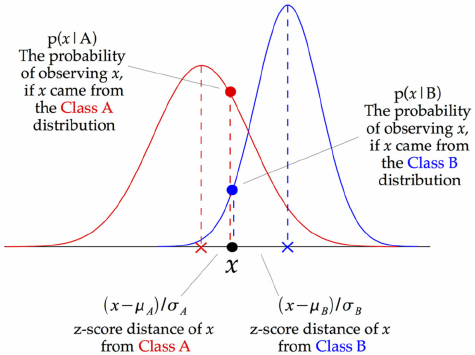
\includegraphics[scale=0.5]{bayes}
\end{figure}
The classifier uses Bayes Theorem, calculates $P(x|A)$ and $P(x|B)$ before making a decision based on the resulting probabilities. This example used one observation with two classes. What happens in the case where you have more than one observation? That's the problem the Naive Bayes classifier solves. 

The classifier assumes that each parameter is independent from the other. Given a set of observations $d$ and a class $c_j$, the probability that $d$ came from $c_j$ is:
\begin{equation}
\label{eq:naivebayes}
P(d|c_j) = P(d_1|c_j) \cdot P(d_2|c_j) \cdot \ldots \cdot P(d_n|c_j)
\end{equation}
which can be simplified to:
\begin{equation}
\label{eq:simnaivebayes}
P(d|c_j) = \prod^{n}_{i=1} P(d_i|c_j)
\end{equation}
This process repeats for all possible classes and the decision is the class with the highest probability. Thus we obtain the following classification rule:
\begin{equation}
\label{eq:classrule}
P(c_j | d_1,\dots,d_n) \propto P(c_j) \prod^{n}_{i=1} P(d_i | c_j) \implies \hat{c} = arg\max_{c_j}P(c_j)\prod^{n}_{i=1}P(d_i | c_j)
\end{equation}
This rule determines the class $\hat{c}$ by choosing the class that maximizes probability. In this particular case, those classes are winning and losing an election. 

There are several types of Naive Bayes classifiers. The one that we employed is the Guassian Naive Bayes. It's designed for models where the parameters have continuous input. Using this model changes the way we calculate the conditional probability. With continuous input, we assume the probability to lie on a normal distribution. Keeping the same terminology as equation \ref{eq:naivebayes} we find $P(d_i | c_j)$ as such:
\begin{equation}
\label{eq:gaussprob}
P(d_i | c_j) = \dfrac{1}{\sqrt{2\pi\sigma^{2}_{c_j}}}\exp\left(\dfrac{(d_i - \mu_{c_j})^2}{2\sigma^{2}_{c_j}}\right)
\end{equation}
The parameters $\sigma_{c_j}$ and $\mu_{c_j}$ are estimated using maximum likelihood. 

The Naive Bayes is the optimal solution given the constraints of the problem. First, the classification problem means that the optimal solution is either a neural network, logistic regression, or Naive Bayes. The chosen approach has limited the size of our dataset. Instead of the three million tweets, the inputs are the hundred and fifty candidates. For smaller data sets, the Naive Bayes has been shown to outperform other models. Both regression and a neural network in crude terms weight their parameters to produce a final result. To ensure accurate weights, the training data needs to be extensive, something not available to us currently. The Naive Bayes probability based approach will take advantage of an unbiased dataset regardless of its size. 

\section{Implementation Naive Bayes in Python}
\hspace{0.2in}The python library Sci-Kit Learn contains a variety of machine learning models. The machine learning can be imported from Sci-Kit, fitted with training data, and then tested using their predict method. Importing the library is done through the import statement.
\begin{verbatim}
from sklearn.naive_bayes import GuassianNB
\end{verbatim}

The data to train and test the algorithm needs to be imported, split, and organized before any fitting can happen. The dataset has been stored as a CSV, and the pandas package will make importing and organization easy. They are stored in a dataframe, which is a python object that is similar to an excel table. 
\begin{verbatim}
import pandas as pd

pd.read_csv(FILE_NAME)
\end{verbatim}

The dataframe is sliced into data and labels. Data is the parameters that the algorithm will read and weight. These parameters include Tweet Count, Positive Tweets, Average Compound Sentiment Score, etc. Labels are the answers for the algorithm to check itself against. Did the candidate win or lose. To allow the algorithm to process the label, winning is a 1 and losing is a 0. Both the training and testing sets have a data and label variable. 
\begin{verbatim}
train_data = np.asarray(senate.loc[:70, `Count':`Average Compound'])
train_labels = np.asarray(senate.loc[70:, `Winner')])
\end{verbatim}
You'll notice that the inputs to the algorithm are all arrays of integers. Even when dealing with text, data needs to be tokenized or shaped into integers that can be organized into arrays for the algorithm to process. Shaping the information and then understanding the output is on the user. 

Fitting the algorithm is easy. The gaussianNB object has a fit function that takes the training data and labels as input.
\begin{verbatim}
gnb = GaussianNB()
gnb.fit(train.data, train.labels)
\end{verbatim}

The algorithm is now trained. To evaluate, use the predict function on the testing set. The predict function will output the prediction, and not the conditional probabilities. To see those, use the predict\_proba function. 
\begin{verbatim}
output = gnb.predict(test_data)
probs = gnb.predict_proba(test_data)
\end{verbatim}
With the ability to predict, we can now evaluate the effectiveness of Naive Bayes. 
 
\section{Evaluating the Model}
\hspace{0.2in} Evaluating a model with just accuracy doesn't capture the full picture of how effective a machine learning model is. It is important to examine subsets of the results to understand how the model interacts with specific classifications. To do this, we use the confusion matrix. 

\begin{figure}[H]
\label{fig:confmatrix}
\centering
	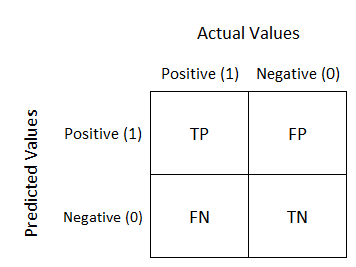
\includegraphics[scale=0.5]{confusion_matrix}
\end{figure}

The confusion matrix outlines the four potential outcomes for any prediction - true/false positives and true/false negatives. These have been used in the medical field for decades when assessing false positives, and gained popularity in machine learning in the 1980's. 

\subsection{Criteria}
\label{subsec:criteria}
\hspace{0.2in} The confusion matrix provides the base for four criteria to evaluate the model. These are precision, accuracy, recall, and f1.

Precision is the ratio of true positives to the sum of true positives and false positives. This is a metric of how often the model is right given that it predicts a candidate to win. It's an important metric because it evaluates the power of the model in regards to predicting a winner. 

\begin{equation}
\label{eq:precision}
PRECISION = \dfrac{TP}{TP+FP}
\end{equation}

Recall is the ratio of true positives to the sum of true positives and false negatives. It's a good measure of how well the algorithm covers actual positive values. 

\begin{equation}
\label{eq:recall}
RECALL = \dfrac{TP}{TP+FN}
\end{equation}

Accuracy is the ratio of true positives to total items in the test set, It's an overall measure of how good the model is. On it's own it's an incomplete metric, but it fits in quite well with the other four. 

\begin{equation}
\label{eq:accuracy}
ACCURACY = \dfrac{TP+TN}{TP+TN+FP+FN}
\end{equation}

Last, the f1 score is the weighted average of the precision and recall. It takes false positives and false negatives into account. 

\begin{equation}
\label{eq:f1}
F1 = 2 \cdot \dfrac{PR \cdot RE}{PR + RE}
\end{equation}

\subsection{Performance}
\hspace{0.2in} To test the model, the data is split into training and testing. First the rows are shuffled and then 75\% of the data goes to training while the other 25\% goes to testing. Here is the resulting confusion matrix from that aplit:
\begin{center}
\begin{tabular}{|c|c|c|}
	\hline
	Predicted/Actual & Positive & Negative \\
	\hline
	Positive & 3 & 8 \\
	\hline
	Negative & 1 &  26\\
	\hline
\end{tabular}
\end{center}
From those, we can calculate the metrics outlined in Section \ref{subsec:criteria}:
\begin{center}
\begin{tabular}{|c|c|}
	\hline
	Metric & Score \\
	\hline
	Precision & 0.75 \\
	\hline
	Accuracy & 0.763\\
	\hline
	Recall & 0.33 \\
	\hline
	F1 & 0.458 \\
	\hline
\end{tabular}
\end{center}

These results are encouraging - particularly the positive precision. Essentially, when the model does decide to predict a positive result, it is likely to be right. It's clear that the model we've implemented is conservative. The significant number of false negatives combine with the low number of false positives shows that the model only predicts positive when a significant amount of evidence shows it to be true. 

The weak recall is potentially a reaction to class imbalance. The negative prediction rate is 0.76. If a larger test set with better balance was included, the greater number of true positives would push the recall higher. 

\end{document}

